% --- capítulo1.tex ---

\chapter{Introducción}

% ===== CONTENIDO REAL DEL CAPÍTULO =====

\section{Estructura del documento (COMPLETAR CUANDO ESTÉ LA DOCUMENTACIÓN)}
En esta sección se encuentran los contenidos de este documento. Aquí se resume brevemente el objetivo de cada uno de los capítulos que lo componen, de modo que el lector pueda anticipar el contenido y la organización de la memoria.
\begin{itemize}
	\item \textbf{Capítulo 1 - Descripción del proyecto:} Se introduce la aplicación, acotando su alcance funcional, perfiles de usuario y restricciones de diseño para bibliotecas medianas y pequeñas. Asimismo, establece los objetivos del proyecto y su trazabilidad mediante la definición detallada de sus criterios de aceptación.
\end{itemize}

\section{Prólogo}
Las bibliotecas han desempeñado un papel fundamental en múltiples sociedades a lo largo de la historia. Durante siglos, estas han actuado como fuentes primarias de conocimiento al servicio de la humanidad. El concepto de la biblioteca —y sus derivados— ha funcionado como un arca del saber y la memoria colectiva a través del tiempo.

Antes, todo trabajo relacionado con la documentación implicaba una tarea compleja: las bibliotecas no eran sencillas de mantener, y su creación demandaba un nivel de organización y recursos que solo podían asumir grupos amplios y estructurados de personas. No obstante, gracias al desarrollo e integración de herramientas computacionales, construir un sistema de catalogación resulta hoy relativamente accesible. De hecho, desde hace décadas existen programas diseñados para cubrir las distintas necesidades que surgen en la gestión de una biblioteca —aspecto que se abordará en secciones posteriores—.

No obstante, estos sistemas pueden llegar a ser difícilmente comprensibles o aplicables a casos en los que tenemos una biblioteca con un fondo más reducido, dado que los sistemas de gestión de bibliotecas suelen estar preparados para ser escalables y contener una cantidad muy grande de información con la que trabaja una biblioteca, tales como datos de usuarios, ejemplares o préstamos. Las soluciones planteadas por la industria informática tienden a ofrecer recursos de —valga la redundancia— medidas industriales.

No todas las bibliotecas tienen el mismo tamaño, ni el mismo sujeto, ni por tanto las mismas necesidades. El sistema que se presenta en este proyecto está orientado a bibliotecas cuyo fondo es de tamaño mediano-pequeño. Debido a ello, será un sistema de gestión destinado a ser accesible, manejable, robusto y seguro en los entornos necesarios.

Una biblioteca no solamente presta a sus socios libros y recursos, sino que sirve de centro de documentación y archivo. Su propósito fundamental es conservar las ideas a lo largo del tiempo y hacer que la información sea pública y accesible para todos sus socios. 

Siguiendo esta línea de pensamiento, he tomado la decisión de desarrollar este proyecto manteniendo estos principios de accesibilidad y apertura. Es por ello por lo que este software será liberado bajo la Licencia Pública General de GNU (GPL), por lo que cualquier persona será libre de usarlo, modificarlo y distribuirlo libremente. De esta forma, cualquier institución o persona podrá apoyarse en este sistema para implementar una biblioteca de las características descritas, o adaptarlo a sus propias necesidades.

En relación con este enfoque de apertura y el dominio funcional del sistema, la aplicación web ha sido bautizada bajo la denominación de Liber. Este nombre responde a un doble propósito conceptual derivado de su etimología en latín, donde el término convive simultáneamente con dos acepciones esenciales para el proyecto: por un lado, hace referencia directa al "libro" \ como unidad primordial del catálogo que se gestiona y, por otro, evoca la condición de "libre", alineándose con el carácter de código abierto del software.

El presente documento constituye la memoria de mi Trabajo de Fin de Grado. En este se recogen de manera estructurada todos los aspectos relacionados con el desarrollo del sistema.

\section{Motivación}

Este proyecto encuentra su motivación fundamental en la preservación de la información y, por extensión, del conocimiento. La observación directa del funcionamiento de bibliotecas que no dependen de entidades gubernamentales ni de grandes instituciones deja ver una problemática cada vez más real: los sistemas de gestión disponibles ofrecen, generalizadamente, un rendimiento insuficiente o una complejidad desproporcionada para su implantación. Las bibliotecas más pequeñas o gestionadas por equipos reducidos necesitan, por tanto, un sistema de catalogación accesible y gratuito que les permita desempeñar su labor. Es precisamente el cubrir esta necesidad la que motiva el desarrollo del presente trabajo. 

\section{Objetivos generales del trabajo}

El fin de este Trabajo de Fin de Grado consiste en liberar un sistema de gestión de bibliotecas de fondo mediano o pequeño accesible para toda la comunidad, tanto para utilizarlo como para poder modificarlo, generando así una comunidad destinada al mantenimiento y posible ampliación de este sistema.  Este sistema ha sido concebido para ser fácil de entender e implementar, con el objeto de hacer la información y el tratamiento de la misma lo más accesible y manejable posible.

El proyecto desarrollado será destinado a bibliotecas cuyo fondo no sea demasiado grande; será una aplicación contenerizada que se podrá desplegar fácilmente para ser ejecutada en local o la nube; esa decisión será competencia de quien utilice el sistema. Una vez desplegada, se podrá usar para hacer tareas de gestión desde el lado de los bibliotecarios y responsables, para funciones tales como dar de alta (o baja) ejemplares, socios, hacer préstamos, y más acciones en las que se ahondará más adelante. También podrán hacer uso de esta aplicación los socios de la biblioteca; podrán usarla para consultar el catálogo disponible, solicitar un préstamo o darse de alta, por ejemplo. Por supuesto, habrá funciones adicionales para usuarios de tipo administrador, como poder hacer operaciones CRUD sobre toda la base de datos.

La aplicación se ha implementado con Django, un framework basado en Python, aprovechando la sencillez que este entorno ofrece para el desarrollo. Dicha elección busca facilitar la comprensión del código fuente, priorizando la legibilidad —dado que el software se liberará bajo una licencia libre— sobre la eficiencia aislada o la complejidad funcional. Se presta así atención a la relación del usuario o programador con el sistema, aspirando a que cualquier persona con nociones básicas de Python y programación pueda comprender y extender esta aplicación sin grandes dificultades.

La finalidad de este proyecto se puede dividir en los siguientes objetivos:

\begin{table}[H]
	\centering
	\caption{Objetivos generales del Trabajo de Fin de Grado.}
	\label{tab:objetivos_generales}
	\begin{tabularx}{\textwidth}{l X}
		\toprule
		\textbf{ID Objetivo} & \textbf{Nombre Objetivo} \\
		\midrule
		\textbf{OBJ-01} & Diseñar una aplicación web que permita la catalogación y gestión de fondos bibliotecarios medianos-pequeños. \\
		\addlinespace
		\textbf{OBJ-02} & Implementar un sistema seguro y robusto de gestión de usuarios diferenciando tres roles de acceso principales bien definidos; socios, bibliotecarios y administradores. \\
		\addlinespace
		\textbf{OBJ-03} & Automatizar el ciclo de vida de los préstamos, controlando las fechas de inicio, fin, devoluciones, prórrogas y la aplicación de penalizaciones por retraso. \\
		\addlinespace
		\textbf{OBJ-04} & Garantizar tanto la portabilidad como inmutabilidad del sistema mediante la contenerización completa de la aplicación recurriendo a Docker, facilitando el despliegue tanto localmente como en la nube. \\
		\addlinespace
		\textbf{OBJ-05} & Fomentar el software libre y la creación de comunidades de desarrollo mediante la liberación del código fuente bajo la Licencia Pública General de GNU (GPL), priorizando la legibilidad y simplicidad del código. \\
		\addlinespace
		\textbf{OBJ-06} & Consolidar a nivel personal las competencias adquiridas en el transcurso del grado en ingeniería, específicamente en el diseño de bases de datos relacionales, arquitectura de software por capas y despliegue de aplicaciones. \\
		\bottomrule
	\end{tabularx}
\end{table}


Más adelante, en el siguiente capítulo, se expondrán los criterios de aceptación para cada uno de los objetivos generales definidos.


\section{Alcance de la aplicación}
En esta sección se procede a definir los límites de la aplicación; todo aquello 
que se ha dejado tanto dentro como fuera de la misma. Se distingue entre el 
alcance del producto (qué funcionalidades ofrece Liber) y el alcance del 
proyecto (bajo qué condiciones se ha desarrollado).

\subsection{Alcance del producto: funcionalidades incluidas}
La aplicación Liber ha sido ideada para responder a las 
necesidades de gestión y catalogación de las bibliotecas de fondo 
mediano-pequeño, tales como las que podemos encontrar en colegios, 
asociaciones o centros culturales.

Con el fin de delimitar la interacción con el sistema, se han definido los 
siguientes perfiles de usuario atendiendo a su grado de especialización técnica:

\begin{itemize}
	\item \textbf{Personal técnico y operativo (Bibliotecarios y Administradores):}
	Este tipo de usuarios constituyen el núcleo de la gestión de Liber. Dado que interactuarán de manera directa con los módulos de catalogación, control de inventario y el ciclo de vida de los préstamos, se asume que estos usuarios poseen un conocimiento previo de los fundamentos sobre los sistemas de gestión bibliotecaria. Las interfaces destinadas a estos roles priorizan la eficiencia, la integridad de los datos y el acceso a operaciones CRUD complejas.
	
	\item \textbf{Usuarios finales (Socios):} 
	Representan a la comunidad que consume los recursos de la biblioteca. Al no precisar de competencias en biblioteconomía ni estar familiarizados con la catalogación, se les ofrece una interfaz intencionadamente simplificada. El alcance funcional para este perfil se restringe a acciones intuitivas y esenciales, tales como la consulta del catálogo público, la solicitud de reservas y la gestión de su perfil personal.
\end{itemize}

De una forma más concreta, las funcionalidades contempladas dentro del alcance 
del producto son las siguientes:

\begin{itemize}
	\item \textbf{Gestión del catálogo:} alta, modificación, consulta y baja de 
	obras y sus ejemplares físicos asociados.
	\item \textbf{Gestión de socios:} registro de usuarios, asignación de roles 
	(socio, bibliotecario, administrador) y control de penalizaciones.
	\item \textbf{Gestión de préstamos:} registro de préstamos, cálculo automático 
	de fechas de devolución, gestión de prórrogas y penalizaciones por retraso.
	\item \textbf{Catálogo público (OPAC):} consulta y búsqueda del fondo 
	bibliográfico por parte de socios y personal.
	\item \textbf{Despliegue contenerizado:} sistema desplegable mediante Docker, 
	tanto en local como en la nube.
	\item \textbf{Software libre:} liberación del código bajo licencia GPL v3 con 
	documentación que facilite su comprensión y extensión.
\end{itemize}

En última instancia, el propósito comercial y social de Liber es captar la 
atención de administradores, responsables de TI y personal directivo de 
organizaciones que busquen una solución de catalogación robusta, 
eficiente y alineada con la filosofía del software libre.

\subsection{Fuera del alcance: funcionalidades excluidas}
Con el objeto de acotar las expectativas del lector y evitar ambigüedades, 
se listan a continuación las funcionalidades que deliberadamente no forman 
parte de este Trabajo de Fin de Grado:

\begin{itemize}
	\item \textbf{Gestión de recursos electrónicos (ERM):} Liber se centra en 
	fondos físicos. La gestión de licencias de publicaciones electrónicas o 
	plataformas SaaS queda fuera del alcance.
	\item \textbf{Interoperabilidad con estándares bibliotecarios avanzados:} no 
	se implementa la importación ni exportación en formato MARC21/UNIMARC, dado 
	que las bibliotecas objetivo no lo requieren.
	\item \textbf{Préstamo interbibliotecario (ILL):} no se contempla la conexión 
	con redes de bibliotecas ni el intercambio de fondos entre instituciones.
	\item \textbf{Inteligencia artificial:} no se incluyen asistentes de 
	catalogación automática, recomendaciones ni analíticas avanzadas.
	\item \textbf{Aplicación móvil nativa:} la interfaz es web y adaptable, pero 
	no se desarrolla una app específica para dispositivos móviles.
	\item \textbf{Internacionalización completa:} la interfaz y documentación se ofrecen
	inicialmente en español, sin traducción a otros idiomas.
	\item \textbf{Módulo de adquisiciones y presupuestos:} no se gestionan 
	compras, proveedores ni facturación.
\end{itemize}

Estas funcionalidades, aunque presentes en soluciones de mayor envergadura 
como Koha o Alma, no resultan necesarias para el nicho de bibliotecas al que 
se orienta Liber, y su inclusión habría desviado el foco del proyecto.

\subsection{Alcance del proyecto: condicionantes}
Desde el punto de vista del proyecto y no del producto, el alcance de este 
Trabajo de Fin de Grado está condicionado por:

\begin{itemize}
	\item \textbf{Desarrollo individual:} el proyecto ha sido desarrollado por 
	un único alumno, bajo la supervisión del tutor.
	\item \textbf{Limitación temporal:} el desarrollo se ha ajustado a la 
	duración establecida.
	\item \textbf{Recursos técnicos:} se han empleado exclusivamente 
	herramientas de software libre (Django, PostgreSQL, Docker, Git).
\end{itemize}

Con el objeto de esclarecer visualmente las particularidades del proyecto, 
se presenta a continuación un árbol de características, que permite hacerse 
a la idea de lo que será y no será el producto resultante de este trabajo.

\begin{figure}[H]
	\centering
	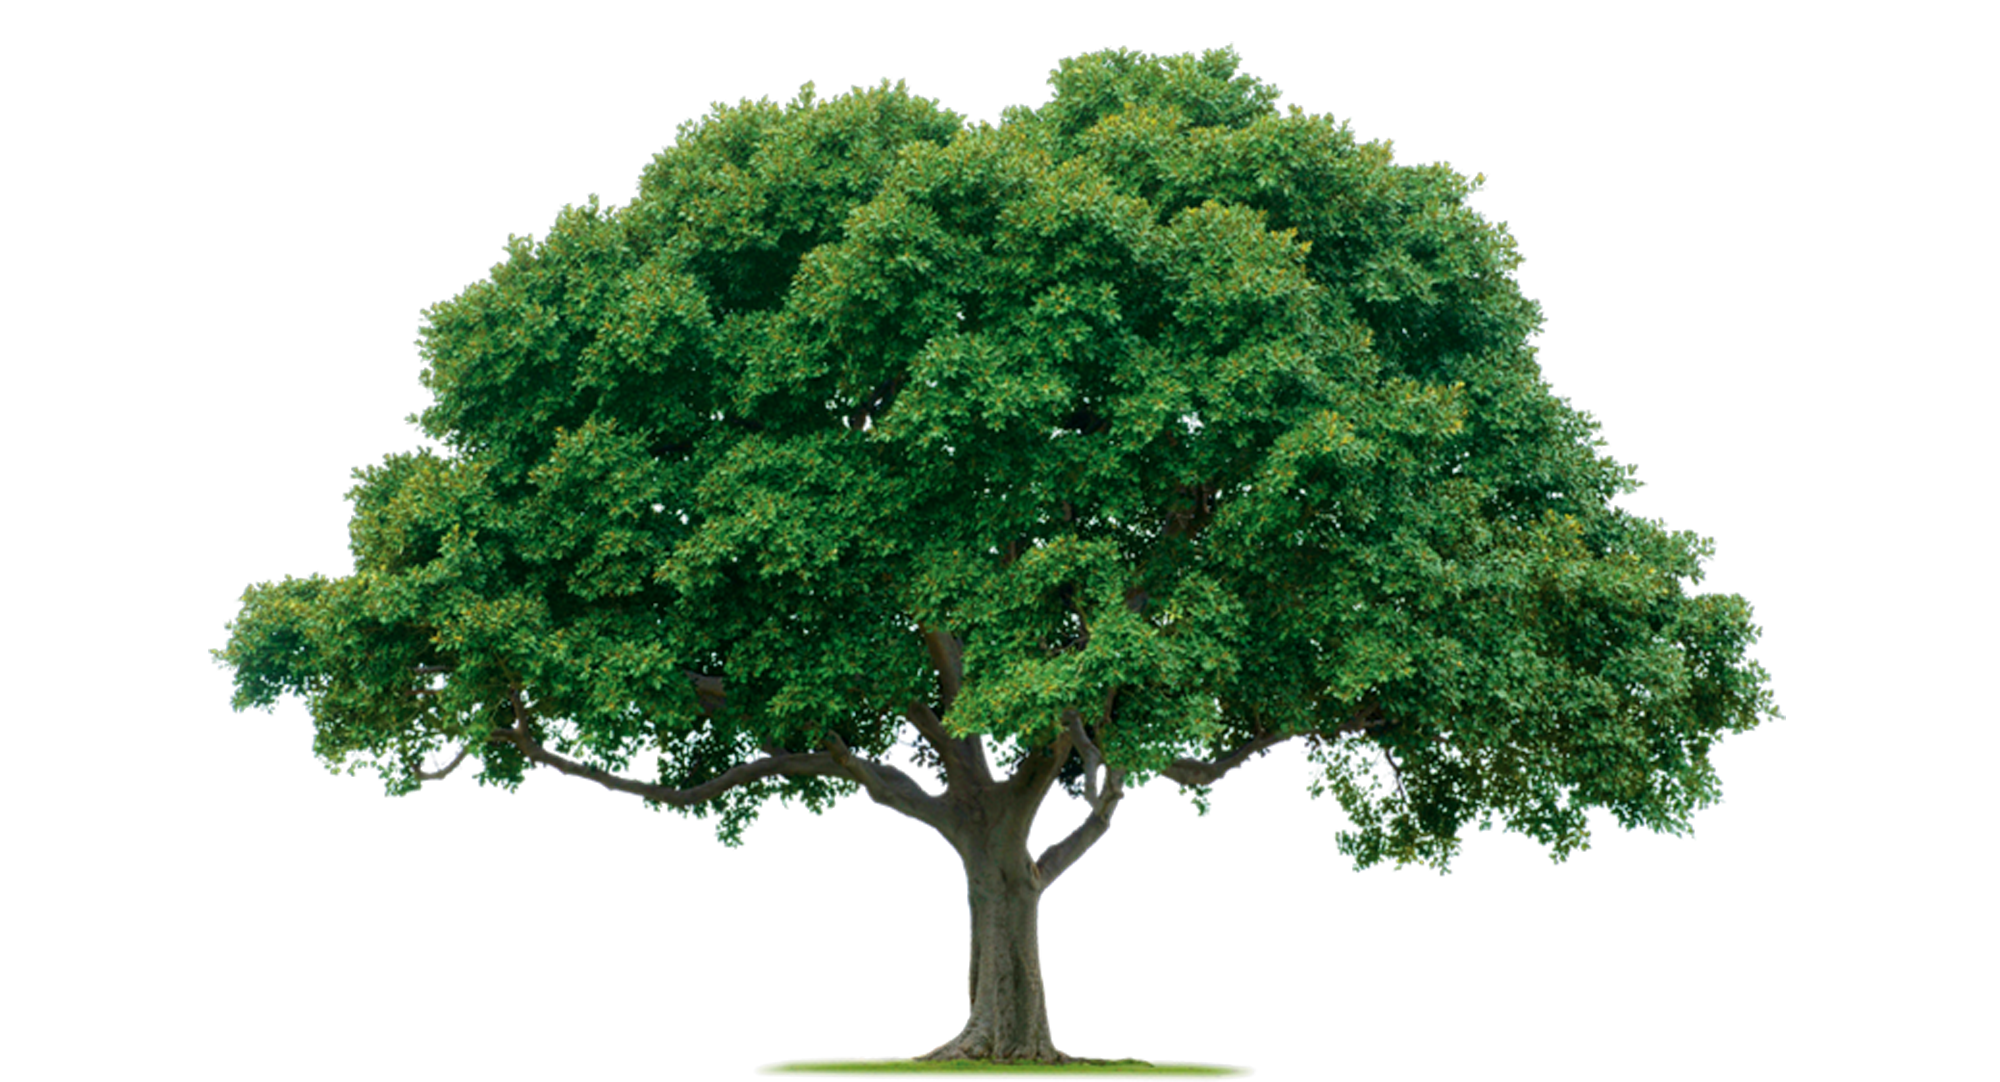
\includegraphics[width=\textwidth]{imagenes/arbol_caracteristicas.png}
	\caption{Árbol de características de Liber.}
	\label{fig:arbol_caracteristicas}
\end{figure}


\subsection{Definición de siglas y abreviaturas}
En este apartado se procede a definir una serie de siglas y expresiones utilizadas para abreviar con el objeto de que la experiencia del lector sea algo más ágil, incluso para aquel que no esté familiarizado con el léxico usado en la memoria.

\begin{table}[H]
	\centering
	\caption{Siglas y abreviaturas empleadas en la memoria.}
	\label{tab:siglas_abreviaturas}
	\begin{tabularx}{\textwidth}{l X}
		\toprule
		\textbf{Sigla / Abreviatura} & \textbf{Significado} \\
		\midrule
		ACID & Atomicity, Consistency, Isolation, Durability (Atomicidad, Consistencia, Aislamiento y Durabilidad) \\
		\addlinespace
		API & Application Programming Interface (Interfaz de Programación de Aplicaciones) \\
		\addlinespace
		CI/CD & Continuous Integration / Continuous Delivery (Integración Continua / Entrega Continua) \\
		\addlinespace
		CRUD & Create, Read, Update, Delete (Crear, Leer, Actualizar, Eliminar) \\
		\addlinespace
		DRY & Don't Repeat Yourself (No te repitas) \\
		\addlinespace
		EAN & European Article Number (Número de Artículo Europeo) \\
		\addlinespace
		ERM & Electronic Resource Management (Gestión de Recursos Electrónicos) \\
		\addlinespace
		GPL & GNU General Public License (Licencia Pública General de GNU) \\
		\addlinespace
		IA & Inteligencia Artificial \\
		\addlinespace
		ILL & Interlibrary Loan (Préstamo Interbibliotecario) \\
		\addlinespace
		ILS & Integrated Library System (Sistema Integrado de Gestión Bibliotecaria) \\
		\addlinespace
		ISBN & International Standard Book Number (Número Internacional Normalizado de Libros) \\
		\addlinespace
		JSON & JavaScript Object Notation (Notación de Objetos de JavaScript) \\
		\addlinespace
		MARC & Machine-Readable Cataloging (Catalogación Legible por Máquina) \\
		\addlinespace
		MVT & Model-View-Template (Modelo-Vista-Plantilla) \\
		\addlinespace
		OPAC & Online Public Access Catalog (Catálogo Público de Acceso en Línea) \\
		\addlinespace
		ORM & Object-Relational Mapping (Mapeo Objeto-Relacional) \\
		\addlinespace
		PSB & Plataforma de Servicios Bibliotecarios \\
		\addlinespace
		SaaS & Software as a Service (Software como Servicio) \\
		\addlinespace
		SIGB & Sistema Integrado de Gestión Bibliotecaria \\
		\addlinespace
		SQL & Structured Query Language (Lenguaje de Consulta Estructurado) \\
		\addlinespace
		TFG & Trabajo de Fin de Grado \\
		\addlinespace
		UML & Unified Modeling Language (Lenguaje Unificado de Modelado) \\
		\addlinespace
		WMS & WorldShare Management Services \\
		\bottomrule
	\end{tabularx}
\end{table}